
\chapter{El m'etodo de la  ecuaci'on de Boltzmann en redes}





\section{Introducci'on}
El m'etodo de la ecuaci'on de Boltzmann en redes (EBR) ha mostrado en los 'ultimos a~nos, ser una herramienta
computacional confiable para realizar simulaciones de problemas de hidrodin'amica~\cite{suc97a,suc01}. 
Con la EBR se han simulado problemas cl'asicos como el de Rayleigh--B'enard~\cite{shan97,inamuro02}, 
magnetohidrodin'amica~\cite{che91}, flujo a trav'es de obst'aculos~\cite{koch97,li04}, sedimentaci'on de part'iculas 
s'olidas~\cite{ladd94,aidun03,ding03b}, propagaci'on de ondas de s'onido~\cite{buick98,buick00}
y  turbulencia~\cite{lockard02}. 
En la presente tesis presentamos resultados de la simulaci'on num'erica de la levitaci'on de una
part'icula circular bidimensional en un campo ac'ustico usando el m'etodo de la ecuaci'on de Boltzmann en
redes.


En este cap'itulo presentamos  brevemente el m'etodo de la EBR partiendo de la ecuaci'on
de transporte de Boltzmann. 'Esta describe la evoluci'on temporal de la funci'on de distribuci'on
de velocidades de una part'icula de un gas dilu'ido. Sabemos que por un m'etodo
perturbativo de la funci'on de distribuci'on en equilibrio, podemos obtener las ecuaciones
de la din'amica de fluidos, por lo que surgi'o la idea de usar la ecuaci'on de transporte
de Boltzmann como una herramienta computacional para el estudio de flujos~\cite{bol98,mcn88,higuera89a}. 
Para esto es necesario discretizar la funci'on de distribuci'on en el espacio, el espacio de velocidades
y el tiempo, con lo que se obtiene el m'etodo de la EBR.
En la secci'on~\ref{sec:etb} presentamos la ecuaci'on de transporte de Boltzmann con el
t'ermino de colisi'on y la hip'otesis de caos molecular establecida por Boltzmann.
En la secci'on~\ref{sec:ebr} presentamos la ecuaci'on
de transporte de Boltzmann discretizada junto con la funci'on de equilibrio para un
espacio de dos dimensiones, que ser'a el usado para el desarrollo de esta tesis.
Demostramos en la secci'on~\ref{sec:hidrodinamica} que podemos llegar a las ecuaciones de la din'amica de fluidos 
para un fluido compresible  a partir de la ecuaci'on de Boltzmann en redes.
Una vez justificado el m'etodo de la EBR presentamos, en la secci'on~\ref{sec:noslip},    las condiciones de frontera
necesarias para simular la levitaci'on ac'ustica. En la siguiente secci'on
describimos lo necesario para simular part'iculas s'olidas en interacci'on con el fluido para la
EBR siguiendo implementaci'on de la interacci'on entre el fluido y la part'icula desarrollada  
por Aidun {\it et al}~\cite{aidun98}.  Finalmente terminamos el cap'itulo con algunas conclusiones.


\section{La ecuaci'on de transporte de Boltzmann}
\label{sec:etb}


Si consideramos un gas monoat'omico formado por $N$ part'iculas  cada una
con masa $m$  y confinadas en un volumen $V$, el estado del gas al tiempo $t$ est'a determinado
por la posici'on $\vr$ y velocidad $\vv$ de cada una de las part'iculas. Dicho gas lo podemos representar
en un espacio de seis dimensiones, tres para la velocidad y las tres restantes para la posici'on, conocido
como el espacio $\mu$, que mostramos esquem'aticamente en la
figura ~\ref{fig:espacio}. La ecuaci'on de transporte de Boltzmann describe el cambio temporal y
espacial de la funci'on de distribuci'on de velocidades $f$ en el espacio $\mu$ que definimos como
\BE
f(\vr,\vv,t) d^3r d^3v = \begin{cases} 
  \text{n'umero promedio de part'iculas que al tiempo $t$ se encuentran  } \\
  \text{en un elemento de volumen $d^3r$ alrededor de $\vr$ con} \\
  \text{velocidades $d^3v$ alrededor de $\vv$.}
  \end{cases}
\EE
En ausencia de colisiones, una part'icula que se encuentra en ($\vr,\vv$) al tiempo $t$
se encontrar'a en $(\vr+\vv \delta t,\vv +(\textbf F/m)\delta t)$
al tiempo $t + \delta t$, siendo $\textbf F$ una fuerza externa actuando sobre el gas.
Entonces podemos escribir
\BE \label{eq:no-colisiones}
f(\vr,\vv,t) d^3r d^3v = f\left(\vr+\vv \delta t,\vv +(\textbf F/m)\delta t,t+\delta t\right) d^3r' d^3v'.
\EE
Si   $\delta t$ es peque~no se puede demostrar que~\cite{kerson63}
\BE
d^3r d^3v = d^3r' d^3v',
\EE
por lo que la ecuaci'on~(\ref{eq:no-colisiones})  la podemos escribir como
\BE\label{eq:f-cero}
f(\vr,\vv,t) = f\left(\vr+\vv \delta t,\vv +(\textbf F/m)\delta t,t+\delta t\right).
\EE


Al tomar en cuenta las colisiones entre part'iculas, la diferencia entre las funciones de distribuci'on
mostrada en la ecuaci'on~(\ref{eq:f-cero}) ya no es cero, por lo que obtenemos
\BE
\label{eq:colision}
f\left(\vr+\vv \delta t,\vv +(\textbf F/m)\delta t,t+\delta t\right) - f(\vr,\vv,t)  = 
\left(\frac{\partial f}{\partial t}\right)_{col}\delta t,
\EE
donde el lado derecho en la ecuaci'on anterior es el t'ermino de colisi'on.
Expandiendo en series de Taylor el lado izquierdo de la ecuaci'on~(\ref{eq:colision})
a primer orden en $\delta t$ obtenemos
\BE\label{eq:taylor-colision}
\left(
\frac{\partial }{\partial t} + \vv \cdot \nabla_{\vr} + \frac{\textbf F}{m}\cdot \nabla_{\vv}
\right) 
f(\vr,\vv,t) = \left(\frac{\partial f}{\partial t}\right)_{col},
\EE
donde
\BE
\nabla_{\vr} = \left(\frac{\partial}{\partial x},\frac{\partial}{\partial y},\frac{\partial}{\partial z} \right),
\qquad 
\nabla_{\vv} = \left(\frac{\partial}{\partial u},\frac{\partial}{\partial v},\frac{\partial}{\partial w} \right),
\EE
$x,y$ y $z$ se refieren a los tres ejes espaciales y $u,v$ y $w$ las componentes de la velocidad para cada uno
de los ejes, respectivamente.
La densidad de part'iculas $n$, la velocidad  $\vu$ y la energ'ia t'ermica $\varepsilon$
son momentos de la funci'on de distribuci'on 
\BE \label{eq:masa}
n(\vr,t) = \int f(\vr,\vv,t) d^3 v %=  m\int f^{eq}(\vr,\vv,t) d^3 v
\EE
\begin{equation}\label{eq:momento} 
\vu (\vr,t)=\frac{1}{n} \int \vv f(\vr,\vv,t) d^3 v. %= \frac{1}{n} \int \vv f^{eq}(\vr,\vv,t) d^3 v
\end{equation}
y
\BE\label{eq:energia}
\varepsilon (\vr,t) = \frac{1}{n} \int \frac{m}{2} (\vv - \vu)^2 f(\vr,\vv,t) d^3 v,
% = \frac{1}{2}  \int (\vv - \vu)^2 f^{eq}(\vv,\vr,t) d^3 v,
\EE
respectivamente, 
donde $\rho=nm$ es la densidad de masa. Boltzmann supuso que el gas es dilu'ido por lo que
su comportamiento termodin'amico debe corresponder a un gas ideal. Por ello, puede definirse una
temperatura local a partir de
\BE
\varepsilon (\vr,t)= \frac{D}{2}nkT,
\EE
donde $D$ es la dimensi'on espacial, $T$ la temperatura local y $k$ la constante de Boltzmann.


\begin{figure}
\centering
%\begin{pspicture}(4,4)
%%\psgrid
%
%\psline[linewidth=.8mm]{->}(0,0)(0,4)
%\psline[linewidth=.8mm]{->}(0,0)(4,0)
%%
%%
%%
%\pscircle[fillstyle=solid,fillcolor=black] (.2,.2){0.05}
%\pscircle[fillstyle=solid,fillcolor=black] (.3,.7){0.05}
%%\pscircle[fillstyle=solid,fillcolor=black] (.5,.3){0.05}
%\pscircle[fillstyle=solid,fillcolor=black] (.9,.5){0.05}
%%\pscircle[fillstyle=solid,fillcolor=black] (.7,.7){0.05}
%%
%%\pscircle[fillstyle=solid,fillcolor=black] (1.2,.2){0.05}
%\pscircle[fillstyle=solid,fillcolor=black] (1.3,.7){0.05}
%\pscircle[fillstyle=solid,fillcolor=black] (1.5,.3){0.05}
%\pscircle[fillstyle=solid,fillcolor=black] (1.9,.5){0.05}
%\pscircle[fillstyle=solid,fillcolor=black] (1.7,.7){0.05}
%%
%%\pscircle[fillstyle=solid,fillcolor=black] (2.2,.2){0.05}
%\pscircle[fillstyle=solid,fillcolor=black] (2.3,.7){0.05}
%\pscircle[fillstyle=solid,fillcolor=black] (2.5,.3){0.05}
%\pscircle[fillstyle=solid,fillcolor=black] (2.9,.5){0.05}
%\pscircle[fillstyle=solid,fillcolor=black] (2.7,.7){0.05}
%%
%\pscircle[fillstyle=solid,fillcolor=black] (3.2,.2){0.05}
%\pscircle[fillstyle=solid,fillcolor=black] (3.3,.7){0.05}
%\pscircle[fillstyle=solid,fillcolor=black] (3.5,.3){0.05}
%%\pscircle[fillstyle=solid,fillcolor=black] (3.9,.5){0.05}
%\pscircle[fillstyle=solid,fillcolor=black] (3.7,.7){0.05}
%%
%
%%
%%
%%
%%\pscircle[fillstyle=solid,fillcolor=black] (.2,1.2){0.05}
%\pscircle[fillstyle=solid,fillcolor=black] (.3,1.7){0.05}
%\pscircle[fillstyle=solid,fillcolor=black] (.5,1.3){0.05}
%%\pscircle[fillstyle=solid,fillcolor=black] (.9,1.5){0.05}
%\pscircle[fillstyle=solid,fillcolor=black] (.7,1.7){0.05}
%%
%\pscircle[fillstyle=solid,fillcolor=black] (1.2,1.2){0.05}
%\pscircle[fillstyle=solid,fillcolor=black] (1.3,1.7){0.05}
%%\pscircle[fillstyle=solid,fillcolor=black] (1.5,1.3){0.05}
%\pscircle[fillstyle=solid,fillcolor=black] (1.9,1.5){0.05}
%\pscircle[fillstyle=solid,fillcolor=black] (1.7,1.7){0.05}
%%
%\pscircle[fillstyle=solid,fillcolor=black] (2.2,1.2){0.05}
%\pscircle[fillstyle=solid,fillcolor=black] (2.3,1.7){0.05}
%%\pscircle[fillstyle=solid,fillcolor=black] (2.5,1.3){0.05}
%\pscircle[fillstyle=solid,fillcolor=black] (2.9,1.5){0.05}
%%\pscircle[fillstyle=solid,fillcolor=black] (2.7,1.7){0.05}
%%
%\pscircle[fillstyle=solid,fillcolor=black] (3.2,1.2){0.05}
%\pscircle[fillstyle=solid,fillcolor=black] (3.3,1.7){0.05}
%%\pscircle[fillstyle=solid,fillcolor=black] (3.5,1.3){0.05}
%\pscircle[fillstyle=solid,fillcolor=black] (3.9,1.5){0.05}
%\pscircle[fillstyle=solid,fillcolor=black] (3.7,1.7){0.05}
%%
%
%%
%%
%%
%%\pscircle[fillstyle=solid,fillcolor=black] (.2,2.2){0.05}
%\pscircle[fillstyle=solid,fillcolor=black] (.3,2.7){0.05}
%%\pscircle[fillstyle=solid,fillcolor=black] (.5,2.3){0.05}
%\pscircle[fillstyle=solid,fillcolor=black] (.9,2.5){0.05}
%\pscircle[fillstyle=solid,fillcolor=black] (.7,2.7){0.05}
%%
%\pscircle[fillstyle=solid,fillcolor=black] (1.2,2.2){0.05}
%\pscircle[fillstyle=solid,fillcolor=black] (1.3,2.7){0.05}
%%\pscircle[fillstyle=solid,fillcolor=black] (1.5,2.3){0.05}
%%\pscircle[fillstyle=solid,fillcolor=black] (1.9,2.5){0.05}
%\pscircle[fillstyle=solid,fillcolor=black] (1.7,2.7){0.05}
%%
%\pscircle[fillstyle=solid,fillcolor=black] (2.2,2.2){0.05}
%\pscircle[fillstyle=solid,fillcolor=black] (2.3,2.7){0.05}
%\pscircle[fillstyle=solid,fillcolor=black] (2.5,2.3){0.05}
%%\pscircle[fillstyle=solid,fillcolor=black] (2.9,2.5){0.05}
%%\pscircle[fillstyle=solid,fillcolor=black] (2.7,2.7){0.05}
%%
%\pscircle[fillstyle=solid,fillcolor=black] (3.2,2.2){0.05}
%\pscircle[fillstyle=solid,fillcolor=black] (3.3,2.7){0.05}
%%\pscircle[fillstyle=solid,fillcolor=black] (3.5,2.3){0.05}
%\pscircle[fillstyle=solid,fillcolor=black] (3.9,2.5){0.05}
%%\pscircle[fillstyle=solid,fillcolor=black] (3.7,2.7){0.05}
%%
%
%%
%%
%%
%\pscircle[fillstyle=solid,fillcolor=black] (.2,3.2){0.05}
%%\pscircle[fillstyle=solid,fillcolor=black] (.3,3.7){0.05}
%\pscircle[fillstyle=solid,fillcolor=black] (.5,3.3){0.05}
%\pscircle[fillstyle=solid,fillcolor=black] (.9,3.5){0.05}
%\pscircle[fillstyle=solid,fillcolor=black] (.7,3.7){0.05}
%%
%\pscircle[fillstyle=solid,fillcolor=black] (1.2,3.2){0.05}
%%\pscircle[fillstyle=solid,fillcolor=black] (1.3,3.7){0.05}
%\pscircle[fillstyle=solid,fillcolor=black] (1.5,3.3){0.05}
%%\pscircle[fillstyle=solid,fillcolor=black] (1.9,3.5){0.05}
%\pscircle[fillstyle=solid,fillcolor=black] (1.7,3.7){0.05}
%%
%%\pscircle[fillstyle=solid,fillcolor=black] (2.2,3.2){0.05}
%\pscircle[fillstyle=solid,fillcolor=black] (2.3,3.7){0.05}
%\pscircle[fillstyle=solid,fillcolor=black] (2.5,3.3){0.05}
%\pscircle[fillstyle=solid,fillcolor=black] (2.9,3.5){0.05}
%%\pscircle[fillstyle=solid,fillcolor=black] (2.7,3.7){0.05}
%%
%%\pscircle[fillstyle=solid,fillcolor=black] (3.2,3.2){0.05}
%%\pscircle[fillstyle=solid,fillcolor=black] (3.3,3.7){0.05}
%\pscircle[fillstyle=solid,fillcolor=black] (3.5,3.3){0.05}
%\pscircle[fillstyle=solid,fillcolor=black] (3.9,3.5){0.05}
%\pscircle[fillstyle=solid,fillcolor=black] (3.7,3.7){0.05}
%%
%
%\psframe[linewidth=0.3mm](2,2.5)(3,3.5)
%\psframe[linewidth=0.2mm,linestyle=dashed](2,0)(3,2.5)
%\psframe[linewidth=0.2mm,linestyle=dashed](0,2.5)(2,3.5)
%\rput[C](-0.4,3){$d^3v$}
%\rput[C](2.5,-.3){$d^3r$}
%\rput[C](0,4.1){$\vv$}
%\rput[C](4.2,0){$\vr$}
%\end{pspicture}
\vskip 2mm
\caption{\label{fig:espacio}
Espacio $\mu$  con $N$ part'iculas de masa $m$. 
}
\end{figure}


Boltzmann encontr'o una forma expl'icita para el t'ermino de colisi'on que es
\BE
\left( \frac{\partial f}{\partial t} \right)_{col} = 
\int \sigma(\Omega) d\Omega \int d^3 v_2 \vert \vv_2 - \vv_1 \vert \left( f_1'f_2'-f_1f_2\right)
\EE
donde $\sigma(\Omega)$ es la secci'on diferencial de choque, 
$\Omega$ es el 'angulo s'olido de dispersi'on  para la colisi'on entre dos part'iculas $f_1$, $f_2$ 
con velocidades $\vv_1$ y $\vv_2$ que tienen  velocidades  $\vv_1'$ y $\vv_2'$ despu'es de 
la colisi'on, respectivamente y $f_1'$ y $f_2'$ son  las funciones de distribuci'on despu'es de la colisi'on. 
Para llegar a esta ecuaci'on Boltzmann consider'o un gas de part'iculas con colisiones  en las cuales
se conserva la masa, la cantidad de movimiento y la energ'ia. Adem'as us'o la hip'otesis
de caos molecular la cual establece la independencia estad'istica de las colisiones binarias.

Se  puede demostrar que una condici'on necesaria y suficiente para alcanzar el equilibrio termodin'amico
en el cual la funci'on de distribuci'on no dependa del tiempo es que
\BE
f'_1 f'_2  = f_1 f_2 = 0.
\EE
De aqu'i obtenemos la funci'on de distribuci'on de velocidades en equilibrio, conocida como la
funci'on de distribuci'on de Maxwell--Boltzmann dada por 
\BE\label{ec:maxwell-boltzmann}
f^{eq} (\vv)= n \left(\frac{m}{2\pi k T}\right)^{D/2} \exp{\left(-\frac{m(\vv-\vu)^2}{2kT}\right)}.
\EE


\section{La ecuaci'on de Boltzmann en redes}
\label{sec:ebr}


En esta secci'on derivamos la ecuaci'on de Boltzmann en redes a partir de la ecuaci'on
de transporte de Boltzmann con la aproximaci'on de  Bhatnagar, Groos y Krook (BGK), discretizando el tiempo y el espacio
de velocidades para obtener la ecuaci'on de Boltzmann en redes para el espacio bidimensional
con nueve velocidades conocido como $D2Q9$.

La ecuaci'on de transporte de Boltzmann es
\BE\label{ec:etb-bgk}
\left(
\frac{\partial }{\partial t} + \vv \cdot \nabla_{\vr} + \frac{\textbf F}{m}\cdot \nabla_{\vv}
\right) 
f(\vr,\vv,t) = \left(\frac{\partial f}{\partial t}\right)_{col},
\EE
donde $f(\vr,\vv,t)$ es la funci'on de distribuci'on y
$\vv$ es la velocidad microsc'opica.

Tomamos la ecuacion~(\ref{eq:colision})  en ausencia de fuerzas de cuerpo
externas obtenemos
\BE\label{eq:t-discreto}
f(\vr+\vv \delta_t,\vv,t+\delta_t) - f(\vr,\vv,t) =
\left(\frac{\partial f}{\partial t}\right)_{col} ,
\EE
y reemplazamos la funci'on de colisi'on por un relajamiento local al equilibrio dado por  
la aproximaci'on BGK~\cite{bgk54,higuera89}
\BE\label{eq:colision-bgk}
\left(\frac{\partial f}{\partial t}\right)_{col} = - \frac{1}{\tau}[f(\vr,\vv,t) -f^{eq}(\vr,\vv,t)]
\EE
donde $\tau$ es el tiempo de relajaci'on adimensional. Las ecuaciones~(\ref{eq:t-discreto})
y~(\ref{eq:colision-bgk}) forman la ecuaci'on de evoluci'on de las funciones de distribuci'on discretizada en el tiempo. 


Si consideramos que la velocidad del gas es cercana a cero,  a la funci'on de distribuci'on de Maxwell--Boltzmann
la podemos escribir en t'erminos de potencias de $\vu$ como
\BE
f^{eq} = \frac{\rho}{(2\pi kT)^{D/2}}\exp\left({-\vv^2/2kT}\right)
\exp\left({\frac{(\vv\cdot\vu)}{kT} - \frac{\vu^2}{2kT}}\right)
\EE
y realizando una expansi'on en series de Taylor alrededor de $\vu =0$
\BE
f^{eq} = 1 + \nabla f^{eq}(0,0) \cdot \vu 
+ \frac{1}{2} \vu \cdot \textbf H(0,0)(\vu)^T + \ldots
 \EE
donde 
\BE
\nabla f^{eq}(0,0) \cdot \vu = \frac{\vv \cdot \vu}{kT}
\EE
y $(\vu)^T$ es la matriz traspuesta de $\vu$ y $\textbf H$ es el hessiano dado por
\BE \textbf H (0,0)=
  \left( 
	\begin{array}{cc}
		-\frac{1}{kT} + \left(\frac{v_x}{kT}\right)^2 &  \left(\frac{v_x}{kT}\right)\left(\frac{v_y}{kT} \right)  \\
	 	\left(\frac{v_y}{kT}\right)\left(\frac{v_x}{kT} \right)& -\frac{1}{kT} + \left(\frac{v_y}{kT}\right)^2
	\end{array},
  \right)
\EE
donde $v_x$ y $v_y$ son los componentes horizontal y vertical de $\vv$.
Evaluando los t'erminos hasta orden $O(\vu^2)$ obtenemos la aproximaci'on para n'umeros de Mach bajos
\BE\label{eq:feq-mach}
f^{eq} = \frac{\rho}{(2\pi kT)^{D/2}}\exp\left(\frac{-\vv^2}{2kT}\right)
\left[
1+\frac{\vv\cdot\vu}{kT}+\frac{(\vv\cdot\vu)^2}{2(kT)^2}-\frac{\vu^2}{2kT}
\right].
\EE


Los momentos hidrodin'amicos de la funci'on de equilibrio los podemos calcular con la siguiente integral
\begin{eqnarray}\label{eq:integral-momentos}
\nonumber
I &=& \int \psi (\vv)f^{eq}d^2v \\ 
\nonumber
&=& \frac{\rho}{(2\pi kT)^{D/2}}\int \psi(\vv) \exp\left(\frac{-\vv^2}{2kT}\right)
\\
\Big[
&1&+\frac{\vv \cdot \vu}{kT}+ \frac{(\vv\cdot\vu)^2}{2(kT)^2}- \frac{\vu^2}{2kT}
\Big]d^2 v.
\end{eqnarray}
donde $\psi(\vv)$ es un polinomio de $\vv$. La integral anterior tiene la forma
\BE
\int e^{-x^2} \psi(x) dx,
\EE
por lo que puede ser calculada num'ericamente usando una cuadratura de Gauss--Hermite
\BE
\label{eq:AB}
\int \psi(\vv) f^{eq}(\vr,\vv,t) d\vv = \sum_\alpha W_\alpha \psi(\vv_\alpha) f^{eq}(\vr,\vv_\alpha,t),
\EE
donde $W_\alpha$ son los coeficientes de la cuadratura Gauss--Hermite y $\vv_\alpha$ es el conjunto
de velocidades discretas. Ahora la masa y la cantidad de movimiento las podemos escribir como
\BE
\rho (\vr,t) = m\sum_\alpha W_\alpha f^{eq}(\vr,\vv_\alpha,t),
\EE
\BE
\vu (\vr,t) = \frac{1}{\rho} \sum_\alpha W_\alpha \vv_\alpha f^{eq}(\vr,\vv_\alpha,t)
\EE
y para la energ'ia
\BE
\varepsilon = \frac{m}{2n} \sum_\alpha W_\alpha | \vv_\alpha-\vu |^2 f^{eq}(\vr,\vv_\alpha,t).
\EE

El polinomio $\psi (\vv)$ tiene la forma
\BE\label{eq:cuadratura}
\psi_{m,n} (\vv) = v^m_xv^n_y.
\EE
Con esto, la ecuaci'on~(\ref{eq:integral-momentos}) es
\begin{eqnarray}
\nonumber
I &=& \int \psi_{m,n}(\vv) f^{eq}d^2 v  \\
\nonumber
&=& \frac{\rho}{2\pi kT} \Big[ \int \int v_x^m v_y^n \exp{(-\eta^2)} \left(1-\frac{u^2}{2kT}\right) dv_x dv_y
\\
\nonumber
&+& \int \int v_x^m v_y^n \exp{(-\eta^2)}\left(\frac{\vv\cdot \vu}{kT} \right) dv_x dv_y
\\
&+& \int \int v_x^m v_y^n \exp{(-\eta^2)}\left( \frac{(\vv \cdot \vu)^2}{2(kT)^2}\right) dv_x dv_y
\Big],
\end{eqnarray}
donde $\eta = v/\sqrt{2kT}$. Al evaluar cada uno de los t'erminos anteriores obtenemos
\begin{eqnarray}
\label{eq:integralota}
 \nonumber
I &=& \int \psi_{m,n}(\vv) f^{eq}d^2 v \\ 
\nonumber
  &=& \frac{\rho}{\pi}\left( \sqrt{2kT}\right)^{m+n}
\Big[\left(1-\frac{\vu^2}{2kT}\right)I_m I_n  \\ 
\nonumber
  &+& \frac{2(u_x I_{m+1}I_n + u_y I_m I_{n+1})}{\sqrt{2kT}} \\
  &+& \frac{u_x^2 I_{m+2}I_n + 2u_xu_yI_{m+1}I_{n+1} + u_y^2I_m I_{n+2}}{kT} \Big],
\end{eqnarray}
donde 
\BE
I_m = \int_{-\infty}^{\infty} e^{-\eta^2}\eta^m d\eta.
\EE 
La ecuaci'on anterior la podemos escribir como la sumatoria de t'erminos de $\eta$ con sus pesos respectivos
\BE\label{eq:B}
I_m = \sum_{j=1}^3 \omega_j \eta^m_j,
\EE
donde  consideramos la suma hasta tercer orden. Al evaluar las sumatorias de la
ecuaci'on~(\ref{eq:B}) en la ecuaci'on~(\ref{eq:integralota}) obtenemos
\BE
I=\frac{\rho}{\pi}\sum_{i,j=1}^3 \omega_j \omega_i \psi (\vv_{i,j})
\left( 1 +\frac{\vv_{i,j}\cdot \vu}{kT} + \frac{(\vv_{i,j}\cdot \vu)^2}{2(kT)^2} - \frac{\vu^2}{2kT} \right).
\EE 
De la ecuaci'on anterior podemos identificar a la funci'on de equilibrio. Para el caso particular de $\psi(\vv)=1$,
la ecuaci'on~(\ref{eq:AB})
\begin{eqnarray}
\nonumber
I &=& \sum_\alpha W_\alpha f^{eq}(\vr,\vv,t) \\
\nonumber
  &=& \frac{\rho}{\pi} \sum_{i,j=1}^3 \omega_i \omega_j 
  \left( 1 +\frac{\vv_{i,j}\cdot \vu}{kT} + \frac{(\vv_{i,j}\cdot \vu)^2}{2(kT)^2} - \frac{\vu^2}{2kT} \right)\\
  &=& \sum_{i,j=1}^3 f^{eq}_{i,j},
 \end{eqnarray}
donde
\BE
f^{eq}_{i,j} =\frac{\omega_i \omega_j}{\pi} \rho \left( 
1 +\frac{\vv_{i,j}\cdot \vu}{kT} + \frac{(\vv_{i,j}\cdot \vu)^2}{2(kT)^2} - \frac{\vu^2}{2kT}\right).
\EE

Para determinar los valores de $\omega_i \omega_j$, empleamos los polinomios de Hermite calculando los valores
de $\eta_i$. Los polinomios son de la forma
\BE
\textbf H (\eta) = (-1)^n e^{\eta^2} \frac{d^n}{d\eta^n}e^{-\eta^2},
\EE
y al resolver para $n=3$ 
\BE
\textbf H_3(\eta) = 8\eta^3 - 12\eta,
\EE
por lo que $\eta_1=-\sqrt{3/2}$, $\eta_2 = 0$ y $\eta_3 = \sqrt{3/2}$.
Finalmente, para encontrar los pesos, utilizamos la formula de Hermite
\BE
\omega_i =\frac{2^{n+1 n\! \sqrt \pi}}{\left[H'_n(\eta_i)\right]^2},
\EE
donde $H'_n$ es la derivada del polinomio de Hermite de orden $n$. Para $n=3$
\BE
H'_3(\eta) = 24\eta^2 - 12,
\EE
entonces $H'_3(\eta_1) = 24$, $H'_3(\eta_2) = -12$ y $H'_3(\eta_3) = 24$, por lo tanto
\BE
\omega_1 = \frac{\sqrt \pi}{6}, \qquad \omega_2 = \frac{2\sqrt \pi}{3} \qquad  \text{y} \qquad \omega_3 = \frac{\sqrt \pi}{6}.
\EE.
Entonces
\BE
w_{\alpha}=\frac{\omega_i\omega_j}{\pi} =\left\{ 
	\begin{array}{lll}
		 4/9, & 	i=j=2, 		& \alpha=0\\
		 1/9, & 	i=1,j=2,...,	& \alpha=1,2,3,4\\
		 1/36,& 	i=j=1,...,  	& \alpha= 5,6,7,8
	\end{array}\right.
\EE
la funci'on de distribuci'on de equilibrio la podemos  escribir como
\BE
f^{eq}_\alpha (\vr,t) = w_\alpha \rho
\left( 1 +\frac{3 (c_\alpha \cdot \vu)} {c^2} + \frac{9( c_\alpha \cdot\vu)^2}{2c^4} 
- \frac{3\vu^2}{2c^2} \right),
\EE
donde 
\begin{equation}
c_\alpha = \left\{
	\begin{array}{lll}
  		(0,0)&   & \alpha =0  \\
 		(\cos\theta_\alpha,\sin\theta_\alpha)c,&       \theta_\alpha=(\alpha -1 )\pi/2,       & \alpha=1,2,3,4 \\
  		\sqrt 2(\cos\theta_\alpha,\sin\theta_\alpha)c,& \theta_\alpha = (\alpha-5)\pi/2+\pi/4,& \alpha =5,6,7,8
	\end{array} 
\right.
\end{equation}
y $c_s^2 = c^2/3$ es la velocidad del sonido y $c= \delta_x/\delta_t$, donde $\delta_x$  es  la distancia 
entre nodo y nodo y usualmente es unitaria y $\delta_t$ es el intervalo de tiempo discretizado, tambi'en unitario.
Entonces la ecuaci'on de Boltzmann en redes  es
\begin{equation}
 \label{eq:bol}
 f_\alpha(\vr +\delta t \vc_\alpha,t+\delta t)-f_\alpha(\vr,t) = \frac{1}{\tau}(f_\alpha^{eq}(\vr,t)-f_\alpha(\vr,t))
\end{equation}
donde $\alpha=0,\ldots,8$ para la malla $D2Q9$, que mostramos en la figura~\ref{fig:d2q9}.





\begin{figure}
\centering
%\begin{pspicture}(3,3)
%%\psgrid
%%
%\psframe[linewidth=0.2mm,linestyle=dashed](0,0)(3,3)
%\psline [linewidth=0.2mm,linestyle=dashed](1.5,0)(1.5,3)
%\psline [linewidth=0.2mm,linestyle=dashed](0,1.5)(3,1.5)
%\psline [linewidth=0.2mm,linestyle=dashed](0,3)(3,0)
%\psline [linewidth=0.2mm,linestyle=dashed](0,0)(3,3)
%\pscircle[fillstyle=solid,fillcolor=black] (0,0){0.1}
%\pscircle[fillstyle=solid,fillcolor=black] (1.5,0){0.1}
%\pscircle[fillstyle=solid,fillcolor=black] (3,0){0.1}
%\pscircle[fillstyle=solid,fillcolor=black] (0,1.5){0.1}
%\pscircle[fillstyle=solid,fillcolor=black] (1.5,1.5){0.1}
%\pscircle[fillstyle=solid,fillcolor=black] (3,1.5){0.1}
%\pscircle[fillstyle=solid,fillcolor=black] (0,3){0.1}
%\pscircle[fillstyle=solid,fillcolor=black] (1.5,3){0.1}
%\pscircle[fillstyle=solid,fillcolor=black] (3,3){0.1}
%\psline[linewidth=0.4mm,linestyle=solid]{->}(1.5,1.5)(1.5,2.8)
%\psline[linewidth=0.4mm,linestyle=solid]{->}(1.5,1.5)(1.5,0.2)
%\psline[linewidth=0.4mm,linestyle=solid]{->}(1.5,1.5)(0.2,1.5)
%\psline[linewidth=0.4mm,linestyle=solid]{->}(1.5,1.5)(2.8,1.5)
%\psline[linewidth=0.4mm,linestyle=solid]{->}(1.5,1.5)(2.8,2.8)
%\psline[linewidth=0.4mm,linestyle=solid]{->}(1.5,1.5)(2.8,0.2)
%\psline[linewidth=0.4mm,linestyle=solid]{->}(1.5,1.5)(0.2,2.8)
%\psline[linewidth=0.4mm,linestyle=solid]{->}(1.5,1.5)(0.2,0.2)
%\rput[C](-0.3,0){$\vc_7$}
%\rput[C](-0.3,1.5){$\vc_3$}
%\rput[C](-0.3,3){$\vc_6$}
%
%
%\rput[C](3.3,0){$\vc_8$}
%\rput[C](3.3,1.5){$\vc_1$}
%\rput[C](3.3,3){$\vc_5$}
%
%\rput[C](1.5,3.25){$\vc_2$}
%\rput[C](1.5,-.25){$\vc_4$}
%
%\end{pspicture}
\caption{\label{fig:d2q9}
Esquema de las velocidades $\vc_\alpha$ para la malla  $D2Q9$ con rapideces $0,1$ y $\sqrt 2$. La velocidad
$\vc_0$ se localiza en el centro.
}
\end{figure}



\section{De la ecuaci'on de Boltzmann  en redes a la mec'anica de fluidos}
\label{sec:hidrodinamica}


En esta secci'on presentamos brevemente la deducci'on de  las ecuaciones de Navier--Stokes a partir de la ecuaci'on
de evoluci'on de la EBR usando la expansi'on de Chapman-Enksog~\cite{guo00}, que es 
una expansi'on usando un formalismo multiescalas para el tiempo y el espacio. 
Primero realizamos una expansi'on en series de Taylor, s'olo al t'ermino del lado izquierdo
de la ecuaci'on~(\ref{eq:bol})
\begin{eqnarray}
\label{eq:expansion}
\nonumber
f_\alpha (\vr + \vc_\alpha \delta t, t + \delta t) &=& 
f_\alpha (\vr,t) + \epsilon \vc_\alpha \cdot \nabla f_\alpha(\vr,t) 
+ \epsilon \frac{\partial }{\partial t} f_\alpha (\vr,t)  \\
\nonumber
&+& \epsilon^2 \left( \frac{1}{2} \vc_\alpha \vc_\alpha \nabla^2 f_\alpha (\vr,t) 
+ \vc_\alpha \cdot \nabla \frac{\partial f_\alpha(\vr,t)}{\partial t} + \frac{1}{2} \frac{\partial^2}{\partial t^2} \right)\\
&+& O(\epsilon^3),
\end{eqnarray}
donde $\epsilon=l/L$ es el par'ametro de Knudsen definido como el camino libre medio $l$ entre una 
longitud caracter'istica $L$. A segundo orden $\epsilon^2$ tenemos
\begin{eqnarray}
\label{eq:2-28}
\nonumber
\frac{\partial f_\alpha}{\partial t} + \vc_\alpha \cdot \nabla_\vr f_\alpha 
+\epsilon \left( \frac{1}{2}\vc_\alpha \vc_\alpha \nabla^2_\vr f_\alpha
+ \vc_\alpha \cdot \nabla_\vr \frac{\partial f_\alpha}{\partial t} 
+ \frac{1}{2} \frac{\partial^2 f_\alpha(\vr,t)}{\partial_t^2}\right)  \\
=\frac{f_\alpha-f_\alpha^{eq}}{\epsilon \tau}.
\end{eqnarray}
Como dijimos anteriormente, para derivar las ecuaciones hidrodin'amicas empleamos un formalismo multiescalas
en el tiempo y el espacio
\BE
\label{eq:formalismo}
\frac{\partial}{\partial t} = \frac{\partial}{\partial t_1} + \epsilon \frac{\partial}{\partial t_2} + \ldots
\qquad {\text y} \qquad
\frac{\partial}{\partial \vr} = \frac{\partial}{\partial \vr_1 },
\EE
respectivamente, y como veremos  m'as adelante es suficiente a primer orden en el tiempo y a orden cero para 
el espacio para recuperar las ecuaciones hidrodin'amicas. El significado f'isico
de las expansiones anteriores es que el relajamiento local al equilibrio se presenta 
en una escala de tiempo $\epsilon^0$ , mientras que las perturbaciones que se propagan como 
ondas de sonido lo hacen en una escala temporal $\epsilon^{-1}$ 
y los efectos difusivos y  advectivos se presentan en una escala temporal $\epsilon^{-2}$. De la misma
manera, expandemos la funci'on de distribuci'on alrededor del equilibrio local
\BE
\label{eq:2-29}
f_\alpha = f_\alpha^{eq} + \epsilon f_\alpha^{(1)} + \epsilon^2 f_\alpha^{(2)} + O(\epsilon^3). 
\EE
Los momentos de la funci'on de equilibrio son
\BE
\label{eq:2-30}
\sum_\alpha f_\alpha^{eq} = \rho, \qquad
\sum_\alpha f_\alpha^{eq} \vc_\alpha = \rho \vu.
\EE
Por otro lado, las funciones $f_\alpha^{(k)}$ para $k=1,2$ cumplen que
\BE
\label{eq:2-31}
\sum_\alpha f_\alpha^{(k)} = 0, \qquad
\sum_\alpha f_\alpha^{(k)} \vc_\alpha = 0.
\EE
De la ecuaci'on~(\ref{eq:2-28}), sustituimos el formalismo multiescalas y la expansi'on de la funci'on de equilibrio
dados por las ecuaciones~(\ref{eq:formalismo}) y~(\ref{eq:2-29})  y recolectamos t'erminos a orden $\epsilon^0$ para obtener
\BE
\label{eq:2-32}
\frac{\partial f_\alpha^{eq}}{\partial t_1} + \vc_\alpha \cdot \nabla_{\vr_1} f_\alpha^{eq} 
= - \frac{f_\alpha^{(1)}}{\tau},
\EE
y a orden $\epsilon^{1}$
\begin{eqnarray}
\label{eq:2-33}
\nonumber
\frac{\partial f_\alpha^{(1)}}{\partial t_1} + \frac{\partial f_\alpha^{eq}}{\partial t_2}
+ \vc_\alpha \cdot \nabla_{\vr_1} f_\alpha^{(1)} 
+ \frac{1}{2} \vc_\alpha \vc_\alpha \nabla_{\vr_1}^2 f_\alpha^{eq} \\
+ \vc_\alpha \cdot \nabla_{\vr_1}\frac{\partial f_\alpha^{eq}}{\partial t_1}
+ \frac{1}{2} \frac{\partial^2 f_\alpha^{eq}}{\partial t_1^2} 
= -\frac{f_\alpha^{(2)}}{\tau}.
\end{eqnarray}
Multiplicamos la ecuaci'on~(\ref{eq:2-32}) primero  por $\partial /\partial t_1$ y 
despu'es por $\vc_\alpha \cdot \nabla_{\vr_1}$ y obtenemos
\BE
\label{eq:2-34}
\frac{\partial^2 f_\alpha^{eq}}{\partial t_1^2} + \vc_\alpha \cdot \nabla_{\vr_1} \frac{\partial f_\alpha^{eq}}{\partial t_1} 
= - \frac{\partial f_\alpha^{(1)}}{\tau\partial t_1}
\EE
y
\BE
\label{eq:2-35}
 \vc_\alpha \nabla_{\vr_1}  \frac{\partial f_\alpha^{eq}}{\partial t_1} 
+ \vc_\alpha \vc_\alpha \cdot \nabla_{\vr_1}^2 f_\alpha^{eq} 
= - \frac{1}{\tau} \vc_\alpha \cdot \nabla_{\vr_1},
\EE
respectivamente. Sumamos las ecuaciones~(\ref{eq:2-34}),~(\ref{eq:2-35}) y multiplicamos por $\frac{1}{2}$
\BE
\label{eq:2-36}
\frac{1}{2} \vc_\alpha \vc_\alpha \nabla_{\vr_1}^2 f_\alpha^{eq}
+ \vc_\alpha \cdot \nabla_{\vr_1} \frac{\partial f_\alpha^{eq}}{\partial t_1}
+ \frac{1}{2} \frac{\partial^2 f_\alpha^{eq}}{\partial t_1^2}
= - \frac{1}{2\tau} \left( \frac{\partial f_\alpha^{(1)}}{\partial t_1}
+\vc_\alpha \cdot \nabla_{\vr_1} f_\alpha^{(1)} \right).
\EE
Ahora, a la ecuaci'on~(\ref{eq:2-33}) le restamos la ecuaci'on~(\ref{eq:2-36})
\BE
\label{eq:2-37}
\frac{\partial f_\alpha^{eq}}{\partial t_2} 
+ \left( 1-\frac{1}{2\tau}\right) 
\left[ \frac{\partial f_\alpha^{(1)}}{\partial t_1} + \vc_\alpha \cdot \nabla_{\vr_1} f_\alpha^{(1)} \right]
= - \frac{f_\alpha^{(2)}}{\tau}.
\EE

Para obtener la ecuaci'on de conservaci'on de masa, multiplicamos la ecuaci'on~(\ref{eq:2-32}) por $\epsilon$, 
realizamos la suma sobre todas las direcciones $\sum_\alpha$  y usamos otra vez el formalismo multiescalas
para obtener
\BE
\label{eq:2-38}
\frac{\partial \rho}{\partial t} + \nabla_{\vr} \cdot \rho \vu = 0.
\EE
La ecuaci'on de la cantidad de movimiento la obtenemos  multiplicando la ecuaci'on~(\ref{eq:2-32}) por $\vc_\alpha$ y
a la ecuaci'on~(\ref{eq:2-37}) por $\epsilon \vc_\alpha$, combinamos ambas ecuaciones y sumamos sobre todas las
direcciones $\sum_\alpha$ para obtener
\BE
\label{eq:2-39}
\frac{\partial \rho \vu}{\partial t} + \nabla_{\vr} \cdot \Pi = 0,
\EE
donde $\Pi$ es el tensor  de momento y tiene la forma
\BE
\label{eq:2-40}
\Pi = \sum_\alpha \vc_\alpha \vc_\alpha \left[ f_\alpha^{eq} 
+ \epsilon\left(1-\frac{1}{2\tau}\right) f_\alpha^{(1)}\right].
 \EE
Al desarrollar la sumatoria sobre las direcciones, el tensor de flujo se puede escribir
como
\BE
\nabla_{\vr} \cdot \Pi = (\vu \cdot \nabla_{\vr}) (\rho \vu) + \nabla_\vr p - \nu \nabla_\vr (\rho \nabla_\vr \vu),
\EE
donde $p=c_s^2\rho$ es la presi'on dada por la ecuaci'on de estado y $\nu = c_s^2(\tau - 1/2)$ es la viscosidad.
Finalmente las ecuaciones de conservaci'on de masa y cantidad de movimiento para un fluido compresible
obtenidas a partir de la ecuaci'on de Boltzmann en redes son
\BE
\frac{\partial \rho}{\partial t} + \nabla_\vr (\rho\vu) = 0
\EE
y
\BE
\frac{\partial (\rho\vu)}{\partial t} + (\vu \cdot \nabla_\vr)\vu = -\nabla_\vr p
+ \nu \nabla_\vr \left(\rho \nabla_\vr \vu\right)
\EE
respectivamente.





 
\section{Condici'on de no deslizamiento y fuerzas de cuerpo externas}
\label{sec:noslip}



Como comentamos en la secci'on~\ref{sec:ebr}, una vez que tenemos la ecuaci'on
de evoluci'on para la ecuaci'on de transporte de Boltzmann, el siguiente paso es
establecer las condiciones de frontera adecuadas para el problema a  simular.
La evoluci'on de la ecuaci'on~(\ref{eq:bol})  la llevamos a cabo en dos pasos,
el relajamiento al equilibrio local, dado por el t'ermino del lado derecho, 
y la propagaci'on de las funciones de distribuci'on
a sus vecino cercanos, como lo indica el t'ermino del lado izquierdo. 
Sin embargo, podemos conceptualizar que
entre el tiempo $t$ y $t+\Delta t/2$ realizamos la relajaci'on al equilibrio local 
y entre el tiempo $t+\Delta t/2$
y $t+\Delta t$ realizamos la propagaci'on.
Es en esta segunda parte cuando aplicamos la condici'on de frontera de no deslizamiento
en las paredes. Para saber en que lugares debemos aplicar la propagaci'on o  la condici'on
de no deslizamiento, donde el fluido tiene la velocidad de la pared,  
es necesario distinguir los nodos de la frontera s'olida con los nodos que son fluido.



\begin{figure}
\centering
%\begin{pspicture}(10,4)
%\psgrid
%
%\psframe[fillstyle=solid,fillcolor=gray](0,0)(4,1)
%%
%\pscircle[fillstyle=solid,fillcolor=black] (0,3){0.1}
%\pscircle[fillstyle=solid,fillcolor=black] (2,3){0.1}
%\pscircle[fillstyle=solid,fillcolor=black] (4,3){0.1}
%%
%\pscircle[fillstyle=solid,fillcolor=black] (2,1){0.1}
%\pscircle[fillstyle=solid,fillcolor=black] (0,1){0.1}
%\pscircle[fillstyle=solid,fillcolor=black] (4,1){0.1}
%%
%\psline[linewidth=0.4mm,linestyle=solid]{->}(2,1)(2,0.2)
%\psline[linewidth=0.4mm,linestyle=solid]{->}(2,1)(3,0.2)
%\psline[linewidth=0.4mm,linestyle=solid]{->}(2,1)(1,0.2)
%%
%\rput[C](2,3.5){$t+\Delta t/2$}
%\rput[C](2,1.3){$\vr$}
%%
%%
%%
%\psframe[fillstyle=solid,fillcolor=gray](6,0)(10,1)
%%
%\pscircle[fillstyle=solid,fillcolor=black] (6,3){0.1}
%\pscircle[fillstyle=solid,fillcolor=black] (8,3){0.1}
%\pscircle[fillstyle=solid,fillcolor=black] (10,3){0.1}
%%
%\pscircle[fillstyle=solid,fillcolor=black] (8,1){0.1}
%\pscircle[fillstyle=solid,fillcolor=black] (6,1){0.1}
%\pscircle[fillstyle=solid,fillcolor=black] (10,1){0.1}
%%
%\psline[linewidth=0.4mm,linestyle=dashed]{->}(8,1)(8,1.8)
%\psline[linewidth=0.4mm,linestyle=dashed]{->}(8,1)(9,1.8)
%\psline[linewidth=0.4mm,linestyle=dashed]{->}(8,1)(7,1.8)
%%
%\rput[C](8,3.5){$t+\Delta t$}
%\rput[C](8,0.7){$\vr$}
%%
%\end{pspicture}
\caption{\label{fig:bounceback}
Esquema del rebote hacia atr'as conocido como bounceback. Al tiempo $t+\Delta t/2$ las funciones
de distribuci'on se encuentran sobre la pared, y al tiempo $t+\Delta t$ invierten su direcci'on.
}
\end{figure}



El rebote hacia atr'as es una condici'on de frontera b'asica para simular la condici'on
de no deslizamiento en paredes. En la figura~\ref{fig:bounceback} esquematizamos  el proceso.
Esta t'ecnica, como mencionamos en el p'arrafo anterior, se aplica entre el tiempo
$t +\Delta t/2$ y $t +\Delta t$  y consiste en invertir la direcci'on de las funciones
de distribuci'on que se encuentran en los nodos de la frontera s'olida y que apuntan
hacia adentro de la pared, como mostramos en la figura. Las funciones de distribuci'on
horizontales, velocidades $\vc_1$ y $\vc_3$ as'i como $\vc_0$, pueden o no invertirse y no
afecta ya que estas funciones no interact'uan con las funciones de distribuci'on de los 
nodos interiores.







\begin{figure}
\centering
%\begin{pspicture}(10,4.5)
%%\psgrid
%%
%\psframe[fillstyle=solid,fillcolor=gray](-.5,0)(4.5,2)
%%
%\pscircle[fillstyle=solid,fillcolor=black] (0,3){0.1}
%\pscircle[fillstyle=solid,fillcolor=black] (2,3){0.1}
%\pscircle[fillstyle=solid,fillcolor=black] (4,3){0.1}
%%
%\pscircle[fillstyle=solid,fillcolor=white] (2,1){0.1}
%\pscircle[fillstyle=solid,fillcolor=white] (0,1){0.1}
%\pscircle[fillstyle=solid,fillcolor=white] (4,1){0.1}
%%
%\psline[linewidth=0.4mm,linestyle=solid]{->}(2,3)(2,2.2)
%\psline[linewidth=0.4mm,linestyle=solid]{->}(2,3)(3,2.2)
%\psline[linewidth=0.4mm,linestyle=solid]{->}(2,3)(1,2.2)
%%
%\rput[C](2,3.3){$\vr$}
%\rput[C](2,4.3){$t+\Delta t/2$}
%%
%%
%%
%%
%
%\psframe[fillstyle=solid,fillcolor=gray](5.5,0)(10.5,2)
%%
%\pscircle[fillstyle=solid,fillcolor=black] (6,3){0.1}
%\pscircle[fillstyle=solid,fillcolor=black] (8,3){0.1}
%\pscircle[fillstyle=solid,fillcolor=black] (10,3){0.1}
%%
%\pscircle[fillstyle=solid,fillcolor=white] (8,1){0.1}
%\pscircle[fillstyle=solid,fillcolor=white] (6,1){0.1}
%\pscircle[fillstyle=solid,fillcolor=white] (10,1){0.1}
%%
%\psline[linewidth=0.4mm,linestyle=dashed]{->}(8,3)(8,3.8)
%\psline[linewidth=0.4mm,linestyle=dashed]{->}(8,3)(9,3.8)
%\psline[linewidth=0.4mm,linestyle=dashed]{->}(8,3)(7,3.8)
%%
%\rput[C](8,2.7){$\vr$}
%\rput[C](8,4.3){$t+\Delta t$}
%%
%%
%%
%%
%\end{pspicture}
\caption{\label{fig:halfway}
Esquema del rebote hacia atr'as a mitad del camino. Al tiempo $t + \Delta t/2$ las funciones
de distribuci'on  que apuntan hacia la pared fantasma invierten su direcci'on para el tiempo 
$t+\Delta t$. 
}
\end{figure}



Otro esquema para recrear la condici'on de no deslizamiento en las paredes es el rebote hacia atr'as
a mitad del camino. La primera diferencia del rebote hacia atr'as a mitad del camino con el explicado
anteriormente, es que los nodos correspondientes a la pared no existen realmente, por lo que suelen
llam'arseles nodos fantasmas. El proceso comienza al tiempo $t + \Delta t /2$, cuando las funciones de
distribuci'on han relajado al equilibrio con la funci'on de colisi'on. Para el tiempo 
$t + \Delta t$ s'olo las funciones de distribuci'on que apuntan hacia la pared fantasma se invierten
mientras que el resto se propagan. Dada la din'amica del rebote hacia atr'as a mitad del camino,
se puede decir que la pared se encuentra a la mitad del camino entre la posici'on del nodo fluido
y el nodo fantasma de la pared.


Si deseamos crear una fuente de movimiento en un fluido, lo podemos lograr 
agregando cantidad de movimiento de manera local. Esto lo logramos
agregando un t'ermino a la ecuaci'on de evoluci'on de la EBR, 
\BE
 f_\alpha(\vr +\Delta t \vc_\alpha,t+\Delta t)-f_\alpha(\vr,t) = \frac{\Delta t}{\tau}(f_\alpha^{eq}(\vr,t)-f_\alpha(\vr,t)) 
+ F_\alpha,
\EE
donde $F_\alpha$ es la cantidad de movimiento que agregamos en el sitio $\vr$ deseado en cada una de las
direcciones. Este t'ermino tiene la forma
\BE
F_\alpha = 3 w_\alpha \left( F_0 c_{\alpha x} + F_0 c_{\alpha y} \right),
\EE
donde $F_{0}$ es la cantidad de movimiento agregado y $(c_{\alpha x},c_{\alpha y})$ indica  que la cantidad de movimiento 
se agrega en el eje $x$ 'o $y$.
Podemos demostrar que  este t'ermino no modifica la densidad del fluido
\BE
\sum_\alpha F_\alpha = \sum_\alpha 3 w_\alpha c_{\alpha x}F_0 +  \sum_\alpha 3 w_\alpha c_{\alpha y}F_0 = 0.
\EE
La contribuci'on a la cantidad de movimiento  para los ejes $x$ y $y$ es
\BE 
\sum_\alpha c_{\alpha x}  F_\alpha = 3F_0\sum_\alpha c_{\alpha x}^2 w_\alpha 
= 3F_0  \left(\frac{2}{9}+\frac{4}{36}\right)= F_0,
\EE
y 
\BE 
\sum_\alpha  c_{\alpha y}  F_\alpha = 3F_0\sum_\alpha c_{\alpha y}^2 w_\alpha 
= 3F_0  \left(\frac{4}{36}+\frac{2}{9}\right)= F_0,
\EE
respectivamente.







\section{Transporte de part'iculas s'olidas en la EBR}
\label{sec:particula}


En esta secci'on presentamos la implementaci'on de part'iculas s'olidas  en movimiento
para el m'etodo de la ecuaci'on de Boltzmann en redes. Ladd~\cite{ladd94}  fue el primero
en desarrollar un m'etodo basado en la EBR para el transporte de 
part'iculas s'olidas suspendidas en un fluido. El m'etodo combina la
din'amica newtoniana de part'iculas s'olidas con la EBR para el fluido. La propuesta de 
Ladd requiere que el fluido cruce la frontera de la part'icula s'olida,
lo que limita la relaci'on de densidad entre la part'icula y el fluido. M'as tarde
Aidun~\cite{aidun98} present'o un m'etodo que supera estos inconvenientes. En esta
secci'on, presentamos solamente el m'etodo desarrollado por Aidun que es el utilizado
en todas las simulaciones num'ericas de esta tesis.

\begin{figure}
\centering
\includegraphics[scale=1.3]{eps/particle.eps}
\caption{\label{fig:particula}
Part'icula de radio $r=5.5$ en la malla $D2Q9$. Los nodos correspondientes a la part'icula
s'olida se marcan con un punto.
}
\end{figure}


El primer paso consiste en dibujar una part'icula dentro de la malla $D2Q9$. En la 
figura~\ref{fig:particula} mostramos un ejemplo de una part'icula circular de 
radio $r=5.5$. Los radios deben ser de la forma  $r= n + 0.5$ donde $n$  es un
n'umero entero  positivo. Esto se debe a que en las fronteras de la part'icula s'olida
con el fluido se utiliza el rebote hacia atr'as a mitad del camino, por lo que la
frontera se encuentra entre nodo y nodo. Ahora comenzamos a llamar a los nodos que
se encuentran dentro de la part'icula como nodos del s'olido (NS) y nodos del fluido (NF) a
aquellos que corresponden al fluido como su nombre lo indica.
Podemos decir que dos nodos cualquiera se conectan mediante un enlace, asociado a la
velocidad $\vc_\alpha$ y estos  enlaces  los podemos clasificar en dos grupos. El primer
grupo,  enlaces entre fluido y fluido (EFF), es aquel conecta a los nodos ubicados en
$\vr$ y $\vr+\vc_\alpha \Delta_t$ y que ambos son fluido. El segundo grupo de enlaces, llamados
enlaces de frontera entre fluido y s'olido (EFS) es aquel que conecta a los nodos ubicados
en $\vr$ y $\vr+\vc_\alpha \Delta t$ y que al menos uno de los dos corresponde a un NS.
Entonces, como dijimos anteriormente, la pared del s'olido se encuentra a la mitad del camino de 
los EFS. La condici'on de no deslizamiento, usando el rebote hacia atr'as a mitad del camino, 
es impuesta a todos los nodos adyacentes a la pared y la podemos  escribir como
\BE
\label{eq:frontera-solido}
  f_\alpha(\vr,t+\Delta t)=\begin{cases}%
       f_{\alpha^{'}}(\vr,t+\Delta t) &\text{si $\vr +\vc_\alpha \Delta t$ es NS},       \\%
       f_\alpha(\vr+\Delta t \vc_\alpha,t+\Delta t),&
        \text{si no},
      \end{cases}
\EE
donde $\alpha'$ se refiere a la direcci'on opuesta a $\alpha$. 
Cuando se usa la ecuaci'on~(\ref{eq:frontera-solido}) el fluido que se encuentra en
$\vr$ al tiempo $t$ realiza un rebote hacia atr'as a mitad del camino si el nodo al que se dirige
corresponde al de un s'olido o se propaga normalmente si corresponde al de un fluido.

Si la pared del s'olido se est'a moviendo con velocidad $\vu_b$, el fluido adyacente a la pared se debe
mover con la misma velocidad. Para todos los nodos de frontera entre el fluido y la pared
se aplica que
\BE
\label{eq:velocidad-ub}	
  f_\alpha(\vr,t+\Delta t)=\begin{cases}%
        f_{\alpha^{'}}(\vr,t+ \Delta t)+2w_\alpha \rho_f \vu_b\cdot \vc_\alpha  &\text{si $\vr + \vc_\alpha \Delta t$ es NS},       \\%
	f_\alpha(\vr+\Delta t \vc_\alpha,t+\Delta t),&
        \text{si no},
      \end{cases}	
\EE
considerando un choque el'astico con la pared.
En la ecuaci'on~(\ref{eq:velocidad-ub}), $\rho_f$ es la densidad del fluido y $w_\alpha$ son los pesos
asociados a la direcci'on $\alpha$.  

La velocidad $\vu_b$ se obtiene de la posici'on del centro de masa de la part'icula s'olida
$\textbf X(t)$, la velocidad translacional $\textbf U(t)$, y la velocidad angular $\Omega (t)$,
\BE
\vu_b =\textbf U(t) + \Omega(t)\times[\textbf r-\textbf X(t)],
\EE
donde $\textbf r$ es la posici'on donde estamos realizando la actualizaci'on de las funciones
de equilibrio.
El fluido donde existen funciones de distribuci'on con  EFS, tiene un incremento en la cantidad de movimiento
\BE
  \delta P_\alpha =\begin{cases}%
        2\vc_\alpha [f_\alpha(\vr,t+\Delta t)-\rho_f(\vr,t+\Delta t)w_\alpha \vu_b\cdot \vc_\alpha] 
&\text{si $\vr+\vc_\alpha \Delta t$ es NS}, \\%
	0,& \text{si no}.
      \end{cases}	
\EE
y por lo tanto una fuerza es ejercida debida a las funciones de distribuci'on con EFS dada por
\BE
\label{eq:Fcs}
F_{\alpha_{EFS}}(\vr + \Delta t\vc_{\alpha^{'}}/2, t+\Delta t) = -\delta P_\alpha/\Delta t,
\EE
sobre los los nodos cubiertos. El torque debido a esta fuerza es
\BE
\label{eq:Tcs}
\textbf T_{\alpha_{EFS}}(\vr + \Delta t\vc_{\alpha^{'}}/2, t+\Delta t) = \left( \textbf r - \textbf X(t)\right) \times 
F_{\alpha_{EFS}}(\vr + \vc_{\alpha^{'}} + \Delta t/2, t+\Delta t).
\EE

La posici'on de la part'icula s'olida se mueve siempre en un continuo, sin embargo por simplicidad,
las fronteras del s'olido se encuentran siempre a la mitad del camino entre nodo y nodo
y la part'icula se redibuja  cada vez que la posici'on redondeada de la part'icula cambia.
De esta manera, conforme la part'icula se mueve va cubriendo y descubriendo la misma cantidad de
nodos. Cuando la part'icula se mueve intercambia cantidad de movimiento con el fluido,
de manera especial cuando cubre y descubre nodos, entonces un peque~no
impulso de fuerza es aplicada a la part'icula s'olida en el intervalo de tiempo $\Delta t$.  
La fuerza debida a los nodos cubiertos en $\vr$ est'a dada por
\BE
\textbf F_c(\vr + \vc_\alpha \Delta t/2,t+\Delta t)= \sum_\alpha f_\alpha(\vr,t)\vc_\alpha,
\EE
y el torque debido a esta fuerza  es
\BE
\textbf T_c(\vr + \vc_\alpha \Delta t/2, t +\Delta t)= \left( \textbf x - \textbf X(t)\right) \times 
\textbf F_c(\vr+ \vc_\alpha \Delta t/2,t+\Delta t),
\EE
El segundo caso especial de intercambio de cantidad de movimiento con el fluido es
al descubrir nodos, primero hay que asignarles un valor de densidad, que obtenemos con la siguiente
relaci'on
\BE
\rho_f (\vr,t) = \frac{1}{N_b} \sum_{N_b} \rho_f(\vr+\vc_\alpha,t),
\EE
donde $\vr$ es la posici'on del nuevo nodo y $N_b$ es el n'umero de nodos adyacentes al nodo 
descubierto que son fluido. Esta relaci'on establece que la densidad del nuevo nodo es igual
al promedio de sus vecinos. La velocidad macrosc'opica del nuevo nodo es igual a la de la frontera
del s'olido al tiempo que es descubierto, esto es
\BE
\vu (\vr,t) = \textbf U(t) + \Omega(t)\times[\textbf r-\textbf X(t)].
\EE
 Como los nodos creados llevan una cantidad de movimiento, la part'icula s'olida debe perder 
esta cantidad de movimiento, por lo que la fuerza y el torque  debido a los nodos descubiertos 
est'an dados respectivamente por
\begin{eqnarray}
\textbf F_d(\vr + \vc_\alpha \Delta t/2, t+\Delta t) = -\rho_f(\vr,t)\vu(\vr,t)
\end{eqnarray}
y 
\BE
\textbf T_d(\vr + \vc_\alpha \Delta t/2, t+\Delta t) = [\textbf x - \textbf X(t) \times 
\textbf F_d(\vr+\vc_\alpha \Delta t/2, t+\Delta t).
\EE

La fuerza y torque total  ejercida sobre la part'icula s'olida al tiempo $t + \Delta t$ est'a dada por
\begin{eqnarray}
\nonumber 
\textbf F(t+\Delta t) &=& \sum_{\alpha_{EFS}} \textbf F_{\alpha_{EFS}}(\vr+\dfrac{1}{2}\vc_\alpha, t +\Delta t/2)
+ \sum_{c} \textbf F_c (\vr,t+\Delta t/2) \\
&+& \sum_{d} \textbf F_d (\vr,t+\Delta t/2) 
\end{eqnarray}
y
\begin{eqnarray}
\nonumber 
\textbf T(t+\Delta t/2) &=& \sum_{\alpha_{EFS}} \textbf T_{\alpha_{EFS}}(\vr+\dfrac{1}{2}\vc_\alpha, t +\Delta t/2)
+ \sum_{c} \textbf T_c (\vr,t+\Delta t/2) \\ 
&+& \sum_{d} \textbf T_d (\vr,t+\Delta t/2),
\end{eqnarray}
respectivamente, donde $\alpha_{EFS}$ se refiere a los enlaces en la direcci'on $\alpha$ fluido s'olido   y los sub'indices
$c$ y $d$ a los nodos cubiertos y descubiertos, respectivamente.  
Con las fuerza y torque netos calculados con las ecuaciones anteriores podemos determinar
el movimiento de la part'icula s'olida resolviendo la ecuaci'on de Newton
\BE
m \frac{d\textbf U(t)}{dt} = \textbf F(t),
\EE
para el movimiento translacional, y
\BE
\textbf I \cdot \frac{d\Omega(t)}{dt} + \Omega(t)\times [\textbf I\cdot \Omega(t)] = \textbf T(t),
\EE
para el movimiento rotacional de la part'icula s'olida. En las ecuaciones anteriores $m$  es la masa
de la part'icula s'olida y $\textbf I$ es el momento de inercia. 

  
%%%%%%%%%%%%%%%%%%%%%%%%%%%%%%%%%%%%%%%%%%%%%%%%%%%%%%%%%%%%%%%%%%%%%%%%%%%%%%%%%%%%%%%%
%%%%%%%%%%%%%%%%%%%%%%%%%%%%%%%%%%%%%%%%%%%%%%%%%%%%%%%%%%%%%%%%%%%%%%%%%%%%%%%%%%%%%%%%
%%%%%%%%%%%%%%%%%%%%%%%%%%%%%%%%%%%%%%%%%%%%%%%%%%%%%%%%%%%%%%%%%%%%%%%%%%%%%%%%%%%%%%%%
%%%%%%%%%%%%%%%%%%%%%%%%%%%%%%%%%%%%%%%%%%%%%%%%%%%%%%%%%%%%%%%%%%%%%%%%%%%%%%%%%%%%%%%%
%%%%%%%%%%%%%%%%%%%%%%%%%%%%%%%%%%%%%%%%%%%%%%%%%%%%%%%%%%%%%%%%%%%%%%%%%%%%%%%%%%%%%%%%



\section{Conclusiones}


En este cap'itulo demostramos que a partir de la ecuaci'on de Boltzmann en redes
podemos obtener las ecuaciones de Navier--Stokes, lo que justifica su uso como m'etodo
num'erico para realizar simulaciones num'ericas de problemas de hidrodin'amica. Tambi'en
planteamos un esquema num'erico para simular la interacci'on de una part'icula
s'olida libre de moverse con el fluido. Adem'as presentamos como implementar la condici'on
de no deslizamiento en paredes y como agregar cantidad  de movimiento, ambas t'ecnicas
las usamos en el problema de levitaci'on ac'ustica que discutimos en el siguiente cap'itulo.
